\section{Individual Work - Marta Pelivan}

\subsection{Equipment Selection}

In the course of preliminary design phase, equipment selection and trade-off is following all design decisions and is iterated numerous times to yield the best possible technical solution while having the lowest mass.

\subsubsection{Part Catalogue}

During starting phase of the development process, extensive Part Catalogue was created to narrow down equipment selection. Main function of this catalogue is easier trade-off of different parts in further iteration steps. This catalogue includes components such as various valve types, mechanical and electrical pressure regulators, pressure transducers, filters, sensors, tanks and thrusters. When selecting components, main driver is to have European suppliers, lowest mass possible and materials compatible with cryogenic propellants. Final Part List is derived from this catalogue.

\subsubsection{Final Part List}

As already shown in Table \ref{tab:equ-lis}, most of the components are from Europe excluding pressure regulator, pressure transducer, filters and thermocouples. Some of these components are also available in Europe but are lacking of technical information required for calculation within this development process. Furthermore, some of European component materials are not compatible with cryogenic propellant. To be able to account mass of each and every component and gain as precise as possible mass budget of the spacecraft, decision was made to include rather non European components during preliminary design. In the upcoming design phases, non European components shall be replaced with European, once all required data is collected. Table \ref{tab:equ-lis} also shows the masses and margins of every component. For the pipes, according to ESA margin philosophy \cite{ESA.2012}, margin of 20\% applies and accounts for transition joints used to enable welded connections between components, such as valves manufactured from titanium alloys, and pipes which are manufactured from stainless steel. Complete part list including materials and links of every part is shown in Table \ref{tab:equ-lis}

\subsection{Propulsion Architecture}

The baseline design of the chemical propulsion system shown in Figure \ref{fig:flow-biprop} consists of two parts:
\begin{itemize}
    \item {Pressurization segment: Two pressurization tanks storing helium.}
    \item{Propellant segment: One fuel tank storing MMH and two oxidizer tanks storing MON-3.}
\end{itemize}
From the given propulsion flow chart it is visible that the system is pressure regulated. Trade-off between pressure regulated and blow-down was performed. Pressure regulated system was selected because of the constant specific impulse and thrust and simpler controlled logic even though the design complexity, and therefore, mass is increasing. Using pressure regulated system brings drawback of additional leakages and failures but they will be mitigated applying redundant components. The main drawback of the blow-down mode is specific impulse and thrust decrease with feed pressure which is not desirable for this type of the mission.
Two assumptions are applied on the baseline design: tanks are filled on the ground using Fill and Drain Valved (FDV) and immediately after filling, purging of the system is done. Pressurization branches of two helium tanks of 40 liters are merged into one branch which features serial pressure regulator from Stanford Mu. Pressure regulator is isolated on the ground with normally closed pyro valves from ArianeGroup, which are fired only once at the start of the engine operation and stays open until the end of operation. Inlet pressure of the pressure regulator is 310 bars, coming from helium tanks, while outlet pressure is 20 bars set by the pressure regulator. Downstream of the helium tanks High Pressure Transducer (HPT1), from Bradford Space, is placed to access the fluidic system and monitor it for possible leakage and calculation of the remaining helium. After PR1 and its isolation PV2, pressurization segment is split into two branches, one for fuel tank and other for oxide tank. Two
check valves in each branch (CV1, CV2, CV3, CV4) are ensuring helium flow only downstream and preventing
propellant mixtures upstream the tanks. Right before propellant tank inlets, one normally closed pyro valve is placed (PV3, PV4) to isolate propellants fumes in the tanks,so that they are not flowing upstream, which would lead to explosion and therefore end of operation.Having a redundant check valves and additional normally closed pyro valves should be investigated in detail in upcoming development stages to asses the need for 5 (e.g. PV2, CV1, CV2, SV1 and PV3) valves between PR1 and tank. As for now, SV1 and SV2 are placed in each branch in case of malfunction or failure of the PR1. Safety valves shall relief the system in case of over pressurisation while the possible torque generated by relief of helium, in the direction outwards of the SV1 and SV2, is not accounted for in the calculations. Pressurisation segment between PR1 and propellant tanks is of critical importance for system functioning throughout the whole mission and therefore, providing with multiple barriers and redundancy should be traded against disadvantages, such as mass and complexity of the system. Upstream the propellant tanks, Low Pressure Transducers (LPT1, LPT2) are monitoring pressurized helium and and detecting if any leakage occurred. 
Downstream PV3 and PV4 in each branch, three propellant tanks are accommodated, one MMH tank of 331 liters and two MON-3 tanks of 198 liters. MMH tank is placed in the main axis of the spacecraft and two MON-3 on each side of MMH in y axis so that the of mass is shifting only along one axis. Downstream the propellant tanks LPT3 and LPT4 are monitoring the propellant flow. Propellant segment is divided into two separate branches with different equipment, one for main engine propellant supply and one for RCS propellant supply. RCS thrusters S10-12 chosen are dual seat, meaning they are incorporating two flow control valves to regulate propellant flow and pressure right before entering combustion chamber. 

\begin{table*}[h]
\centering
\caption{Bipropellant Part List}
\label{tab:equ-lis}
\resizebox{\textwidth}{!}{%
\begin{tabular}{|l|l|r|r|r|r|r|l|} 
\hline
\rowcolor[rgb]{0.553,0.706,0.882} Description                  & Type/Manufacturer                                        & Amount                                                   & \begin{tabular}[c]{@{}>{\cellcolor[rgb]{0.553,0.706,0.882}}r@{}}Mass per~\\unit [kg]\end{tabular} & Margin                               & \begin{tabular}[c]{@{}>{\cellcolor[rgb]{0.553,0.706,0.882}}r@{}}Mass inc.\\margin\end{tabular} & ~ ~ ~ ~ ~ Material~ ~ ~~ & Link                                                                                                                                                                                                                         \\ 
\hline
Pipes                                                          & Pipes                                                    & 1                                                        & 2.540                                                                                             & 0.2                                  & 3.048                                                                                          & Stainless steel          & \href{https://www.pacstainless.com/products/stainless-steel-tubing/304-304l-stainless-steel-tubing/}{Pipes}                                                                                                                                \\ 
\hline
Main Engine                                                    & S400-15                                                  & 1                                                        & 5.200                                                                                             & 0.05                                 & 5.460                                                                                          & Platinum Alloy           & \href{https://www.space-propulsion.com/spacecraft-propulsion/apogee-motors/index.html}{Main Engine}                                                                                                                                             \\ 
\hline
RCS Thruster                                                   & S10-26                                                   & 12                                                       & 1.800                                                                                             & 0.05                                 & 8.190                                                                                          & Platinum Alloy           & \href{https://www.space-propulsion.com/spacecraft-propulsion/bipropellant-thrusters/10-bipropellant-thrusters.html}{RCS Thruster}                                                                                                                 \\ 
\hline
Helium Tank                                                    & PVG Family 40l                                           & 2                                                        & 8.500                                                                                             & 0.05                                 & 18.700                                                                                         & Titanium Alloy           & \href{https://www.mt-aerospace.de/files/mta/tankkatalog/MT-Tankkatalog.pdf}{Helium Tank}                                                                                                                                                       \\ 
\hline
Fuel Tank                                                      & OST 25/0                                                 & 1                                                        & 21.000                                                                                            & 0.05                                 & 22.050                                                                                         & Titanium Alloy           & \href{https://www.space-propulsion.com/spacecraft-propulsion/bipropellant-tanks/index.html\#198}{Fuel Tank}                                                                                                                                   \\ 
\hline
Oxide Tank                                                     & OST 25/0                                                 & 2                                                        & 21.000                                                                                            & 0.05                                 & 44.100                                                                                         & Titanium Alloy           & \href{https://www.space-propulsion.com/spacecraft-propulsion/bipropellant-tanks/index.html\#198}{Oxide Tanks}                                                                                                                                  \\ 
\hline
Fill Drain Valve                                               & ArianeGroup                                              & 3                                                        & 0.060                                                                                             & 0.05                                 & 0.315                                                                                          & Titanium Alloy           & \href{https://www.space-propulsion.com/brochures/valves/space-propulsion-valves.pdf}{FDV}                                                                                                                                          \\ 
\hline
Latch Valve                                                    & ArianeGroup                                              & 4                                                        & 0.545                                                                                             & 0.05                                 & 2.289                                                                                          & Titanium Alloy           & \href{https://www.space-propulsion.com/brochures/valves/space-propulsion-valves.pdf}{LV}                                                                                                                                               \\ 
\hline
Pyro Isolation Valve                                           & ArianeGroup                                              & 16                                                       & 0.160                                                                                             & 0.05                                 & 2.688                                                                                          & Titanium Alloy           & \href{https://www.space-propulsion.com/brochures/valves/space-propulsion-valves.pdf}{PV}                                                                                                                                                \\ 
\hline
Check Valve                                                    & {\cellcolor[rgb]{1,0.831,0.541}}Vacco                    & 4                                                        & 0.020                                                                                             & 0.05                                 & 0.084                                                                                          & Titanium Alloy           & \href{https://www.vacco.com/images/uploads/pdfs/check\_valves.pdf}{CV}                                                                                                                                                                 \\ 
\hline
Safety Relief Valve                                            & Safran                                                   & 2                                                        & 0.700                                                                                             & 0.05                                 & 1.470                                                                                          & /                        & \href{https://www.safran-group.com/products-services/safety-relief-valve-ssei}{SV}                                                                                                                                                      \\ 
\hline
Filter                                                         & {\cellcolor[rgb]{1,0.831,0.541}}Vacco                    & 8                                                        & 1.500                                                                                             & 0.05                                 & 12.600                                                                                         & Stainless steel          & \href{https://www.vacco.com/images/uploads/pdfs/VACCO\_Filtration\_Catalog\_042121\_FINAL\_with\_bookmarks\_web.pdf}{Filter}                                                                                                                \\ 
\hline
Dual Pressure Regulator                                        & {\cellcolor[rgb]{1,0.831,0.541}}Stanford Mu              & 1                                                        & 1.130                                                                                             & 0.05                                 & 1.187                                                                                          & /                        & \href{https://stanfordmu.com/feature-works/}{PR}                                                                                                                                                                                        \\ 
\hline
Pressure Transducer                                            & {\cellcolor[rgb]{1,0.831,0.541}}Bradford Space           & 5                                                        & 0.230                                                                                             & 0.05                                 & 1.207                                                                                          & Titanium Alloy           & \href{https://static1.squarespace.com/static/603ed12be884730013401d7a/t/6054f46fbaf06f76bbaba605/1616180337738/be\_datasheet\_sapt\_2019oct.pdf}{PT}                                                                                    \\ 
\hline
Thermocouples                                                  & {\cellcolor[rgb]{1,0.831,0.541}}Collins Aerospace        & 12                                                       & 0.350                                                                                             & 0.05                                 & 4.410                                                                                          & /                        & \href{https://prd-sc101-cdn.rtx.com/-/media/ca/product-assets/marketing/s/space/model-0118mf-high-reliability-surface-temperature-sensor-data-sheet.pdf?rev=64b96706e03f4d20a9c3f8dbc54e0fe4hash=FA6A53CD201F49CFC49B4DFBAA274200}{Thermocouples}  \\ 
\hline
\multicolumn{1}{|l}{{\cellcolor[rgb]{0.773,0.851,0.941}}Total} & \multicolumn{1}{l}{{\cellcolor[rgb]{0.773,0.851,0.941}}} & \multicolumn{1}{r}{{\cellcolor[rgb]{0.773,0.851,0.941}}} & \multicolumn{1}{r}{{\cellcolor[rgb]{0.773,0.851,0.941}}}                                          & {\cellcolor[rgb]{0.773,0.851,0.941}} & {\cellcolor[rgb]{0.773,0.851,0.941}}126.948                                                    & \multicolumn{1}{r}{}     & \multicolumn{1}{l}{}                                                                                                                                                                                                         \\ 
\cline{1-6}
\multicolumn{1}{l}{}                                           & \multicolumn{1}{l}{}                                     & \multicolumn{1}{r}{}                                     & \multicolumn{1}{r}{}                                                                              & \multicolumn{1}{r}{}                 & \multicolumn{1}{r}{}                                                                           & \multicolumn{1}{r}{}     & \multicolumn{1}{l}{}                                                                                                                                                                                                         \\
\multicolumn{1}{l}{}                                           & \multicolumn{1}{l}{}                                     & \multicolumn{1}{r}{}                                     & \multicolumn{1}{r}{}                                                                              & \multicolumn{1}{r}{}                 & \multicolumn{1}{r}{}                                                                           & \multicolumn{1}{r}{}     & \multicolumn{1}{l}{}                                                                                                                                                                                                         \\
\multicolumn{1}{l}{}                                           & \multicolumn{1}{l}{}                                     & \multicolumn{1}{r}{}                                     & \multicolumn{1}{r}{}                                                                              & \multicolumn{1}{r}{}                 & \multicolumn{1}{r}{}                                                                           & \multicolumn{1}{r}{}     & \multicolumn{1}{l}{}                                                                                                                                                                                                         \\
\multicolumn{1}{l}{}                                           & \multicolumn{1}{l}{}                                     & \multicolumn{1}{r}{}                                     & \multicolumn{1}{r}{}                                                                              & \multicolumn{1}{r}{}                 & \multicolumn{1}{r}{}                                                                           & \multicolumn{1}{r}{}     & \multicolumn{1}{l}{}                                                                                                                                                                                                        
\end{tabular}}
\end{table*}





Since there are already two valves upstream thrusters, only one additional latch valve is placed to gain at least three barriers to prevent accidental
firing of thrusters, as well as leaking of hazardous fluids. Latch valves are chosen due to their ability to open and close numerous times and can isolate branches where leakage occurs. Adittionally, 2 out of the 12 RCS thrusters can fail and the spacecraft can still operate normally while flow control valves will isolate failed thruster.
As already mentioned, main engine is S400-15 which includes only one solenoid single seat valve so upstream the engine, pyro ladder is introduced. Pyro ladder consists of normally open and normally closed pyro valves placed in such an order that main engine can be isolated three times. First, it is isolated on ground and then PV8 is fired before first maneuver. After the second maneuver, spacecraft is passivated by firing PV7, due to long waiting period between maneuvers and then fired again by PV9 before third maneuver. Last passivation of the main engine is after fifth maneuver by firing PV6, after which main engine is shut-off completely. In case of malfunction of any PV one redundant serially connected normally open and normally closed PV is placed. This process can be followed in Figure \ref{fig:pyro}

\begin{figure}[H]
  \centering
  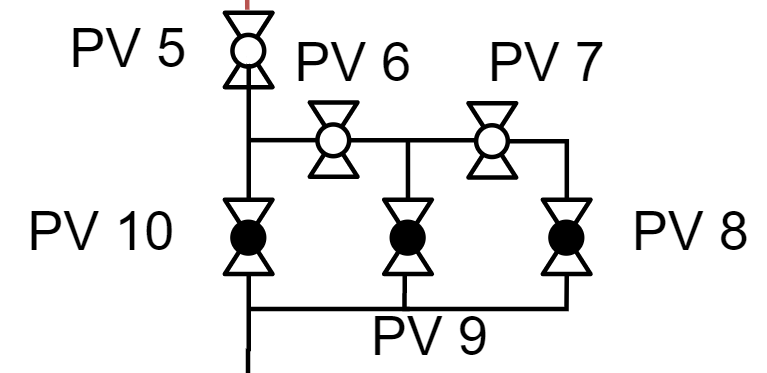
\includegraphics[width=0.7\linewidth]{img/pyroladder.png}
  \caption{Pyro ladder}
  \label{fig:pyro}
\end{figure}


\subsection{Development Support}

\subsubsection{Nuclear Propulsion Research}

At the beginning of design challenge, comprehensive review of nuclear propulsion was done. Even though in the last years interest for nuclear propulsion for interplanetary flight occurred again, there are still not nearly enough information available on the market to make an analysis and calculations needed for this design.

\subsubsection{Pressurant Tank Sizing}


Pressurant tank is sized based on the given calculation from NESC Academy \cite{BottleBl30:online}, but adjusted for the this system requirements. MATLAB script \href{https://github.com/Sven-J-Steinert/MomenTUM/blob/main/MATLAB/pressure_temp_sim.m}{\colorbox{codegray}{pressure\_temp\_sim.m}} takes propellant mass needed per maneuver and time of each maneuver from GMAT. One of the most decisive points would be tank selection which affects volume, mean operating pressure and temperature in the tank. Iteration is done multiple times between tank sizing script and part selection.